\documentclass[a0,landscape]{a0poster}

\usepackage{multicol} 
\columnsep=100pt 
\columnseprule=0pt

\usepackage[svgnames]{xcolor}
\usepackage{graphicx} 
\usepackage{amsfonts, amsmath, amsthm, amssymb}

\usepackage[font=small,labelfont=bf]{caption}

\usepackage{algorithm} 
\usepackage{algpseudocode}

\newcommand {\FlameStream} {FlameStream}

\begin{document}

\begin{minipage}[b]{0.83\linewidth}
  {\veryHuge \color{NavyBlue} \textbf{\FlameStream: Model and Runtime for Distributed Stream Processing}}\\
  \bigbreak
  {\huge \textbf{Igor E. Kuralenok$^1$, Artem Trofimov$^{1,2}$, Nikita Marshalkin$^{1,2}$, and Boris Novikov$^{1,2}$}}\\
  \bigbreak
  {\huge $^1$JetBrains Research, $^2$Saint Petersburg State University}
\end{minipage}
%
\begin{minipage}[b]{0.17\linewidth}
  
\includegraphics[width=20cm]{pics/jetbrains.png} 
\end{minipage}

\vspace{1cm} 

\begin{multicols*}{3}

\begin{abstract}
Exactly-once semantics without high latency overhead is still hard to achieve within state-of-the-art stream processing systems. We introduce a model providing for exactly-once using lightweight optimistic approach for obtaining determinism and idempotence. We show its feasibility with a prototype.
\end {abstract}

\section*{Motivation}

\begin{minipage}{\linewidth}
  \centering
  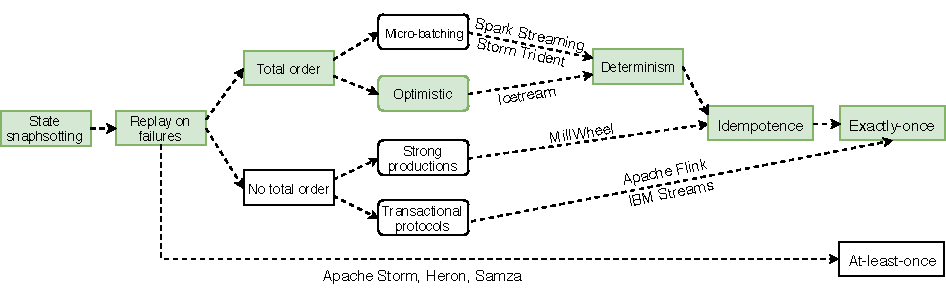
\includegraphics[width=\linewidth]{pics/roadmap}
  \captionof{figure}{The roadmap of approaches for achieving exactly-once and at-least-once guarantees. Green elements indicate the path for our approach}
\end{minipage}

The desired system properties are:

\begin{itemize}
  \item Computational model should be deterministic by design, i.e., it should produce deterministic results for any pipelines and business logic.
  \item The performance overhead should be low in comparison with the existing systems.
\end{itemize}

We will use the following principles for our system:

\begin{itemize}
  \item Support cyclic execution graph
  \item Localize state management in terms of system operation type
  \item A data partition must be processed on a single node
  \item MapReduce completeness
\end{itemize}

\section{Model}

\begin{minipage}{\linewidth}
  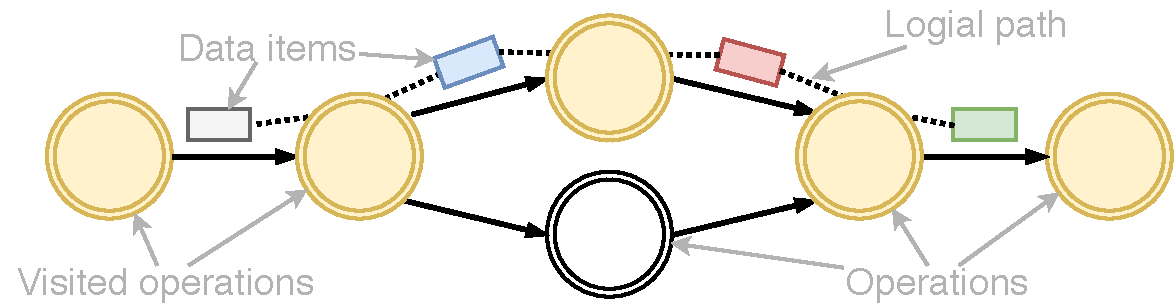
\includegraphics[width=\linewidth]{pics/logical-graph}
  \captionof{figure}{A logical execution graph}
  \label{logical-graph}
\end{minipage}

\begin{minipage}{\linewidth}
  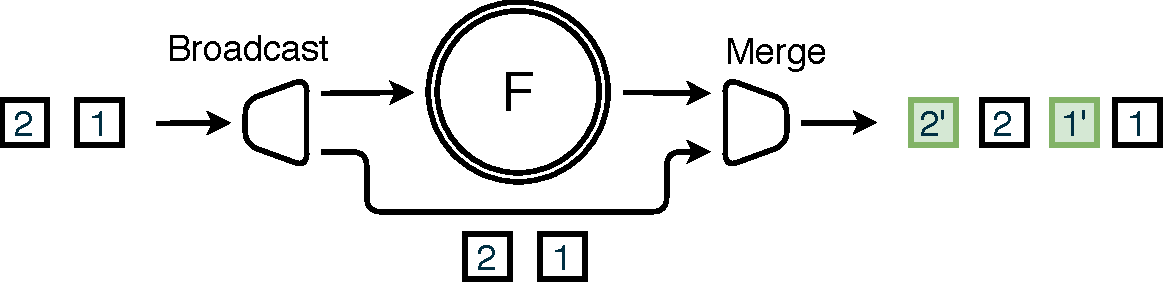
\includegraphics[width=\linewidth]{pics/ordering}
  \captionof{figure}{Ordering model}
  \label{ordering}
\end{minipage}

\begin{minipage}{\linewidth}
  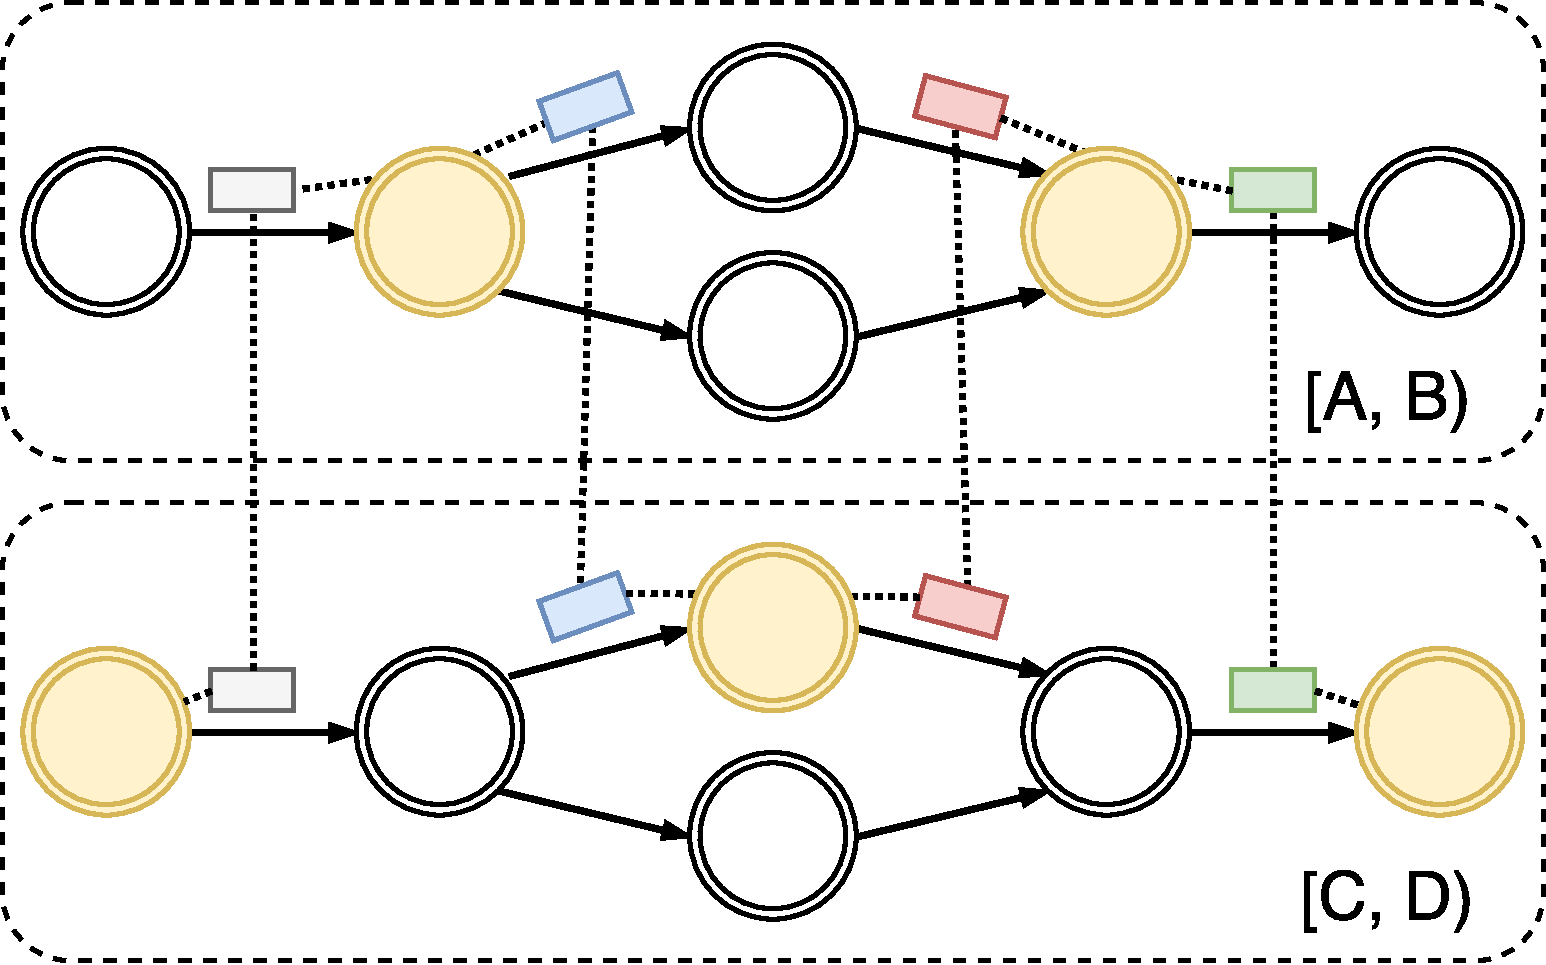
\includegraphics[width=\linewidth]{pics/physical-graph}
  \captionof{figure}{A physical execution graph}
  \label{physical-graph}
\end{minipage}

The list of available operations includes:

\begin{description}
  \item [Map] applies a user-defined function to the payload of an input item and returns a (possibly empty) sequence of data items with transformed payloads. 
  \item [Broadcast] replicates an input item to the specified number of operations.
  \item [Merge] operation is initialized with the specified number of input nodes. It sends all incoming data to the output.
  \item [Grouping] constructs a single item containing a set of consecutive items that have the same value of partition function. The maximum number of items that can be grouped is specified as a parameter  $Window Size.$ 
\end{description}

The following example illustrates  the grouping operation. 
Let the input stream be a series of integers: $ 1,2,3, \ldots$, and the  partition function returns for even numbers and 0 otherwise. If the window is set to 3, the output is 
$$(1), (2), (1|3), (2|4), (1|3|5), (2|4|6), (3|5|7), (4|6|8), \ldots$$

\section*{Drifting state}

\begin{minipage}{\linewidth}
  \begin{algorithmic}
    \Function{reduce}{$key$, $values$}
      \State $accumulator$ \Comment{reduce's state}
      \ForAll{$v \in values$} 
        \State \Call{combine}{$v$, $accumulator$}
      \EndFor
      \State \Return \Call{map}{$accumulator$}
    \EndFunction
  \end{algorithmic}
  \captionof{figure}{Generic reduce stage}
\end{minipage}

\section*{Optimistic}

\begin{minipage}{\linewidth}
  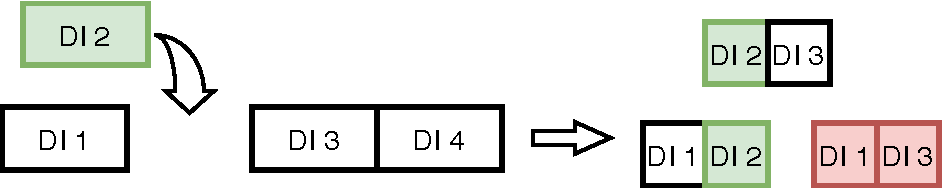
\includegraphics[width=\linewidth]{pics/grouping-replaying}
  \captionof{figure}{The repair in grouping with $WindowSize = 2$.}
  \label {grouping-replaying}
\end{minipage}

\begin{minipage}{\linewidth}
  \centering
  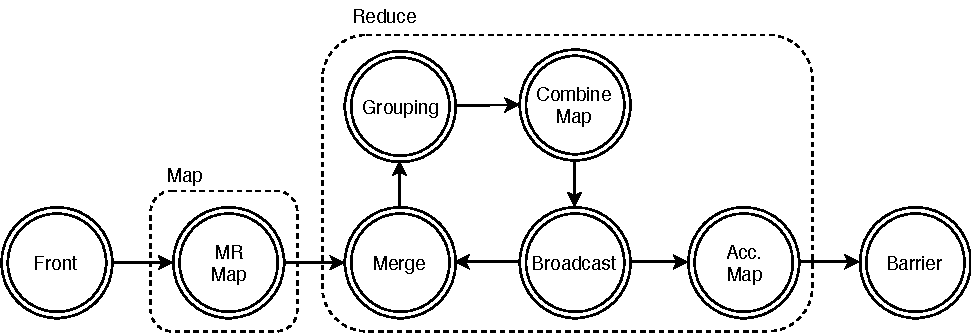
\includegraphics[width=\linewidth]{pics/mapreduce}
  \captionof{figure}{Logical graph for MapReduce transformations}
\end{minipage}

\section*{Implementation}

\[DataItem := (payload, Meta)\]

\[Meta := (GlobalTime, childIds[\:], Trace, isTombstone)\]

\[GlobalTime := (frontTs, frontId)\]

\[Trace := \bigoplus_{op \in \text{visited}} Id(op)\]

\begin{minipage}{\linewidth}
  \centering
  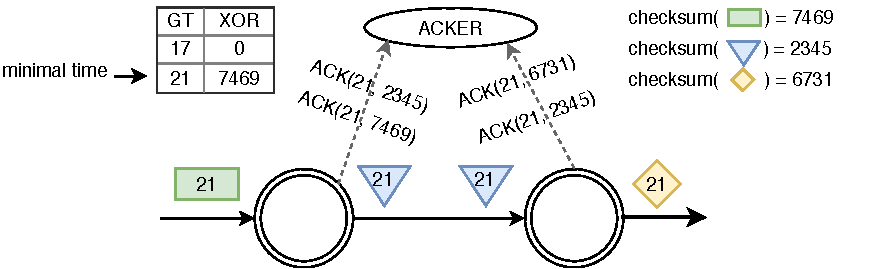
\includegraphics[width=\linewidth]{pics/acker}
  \captionof{figure}{The example of tracking minimal time using acker}
\end{minipage}

\section*{Experiments}

\begin{minipage}{\linewidth}
  \centering
  \begin{minipage}[b]{.58\linewidth}
    \centering
    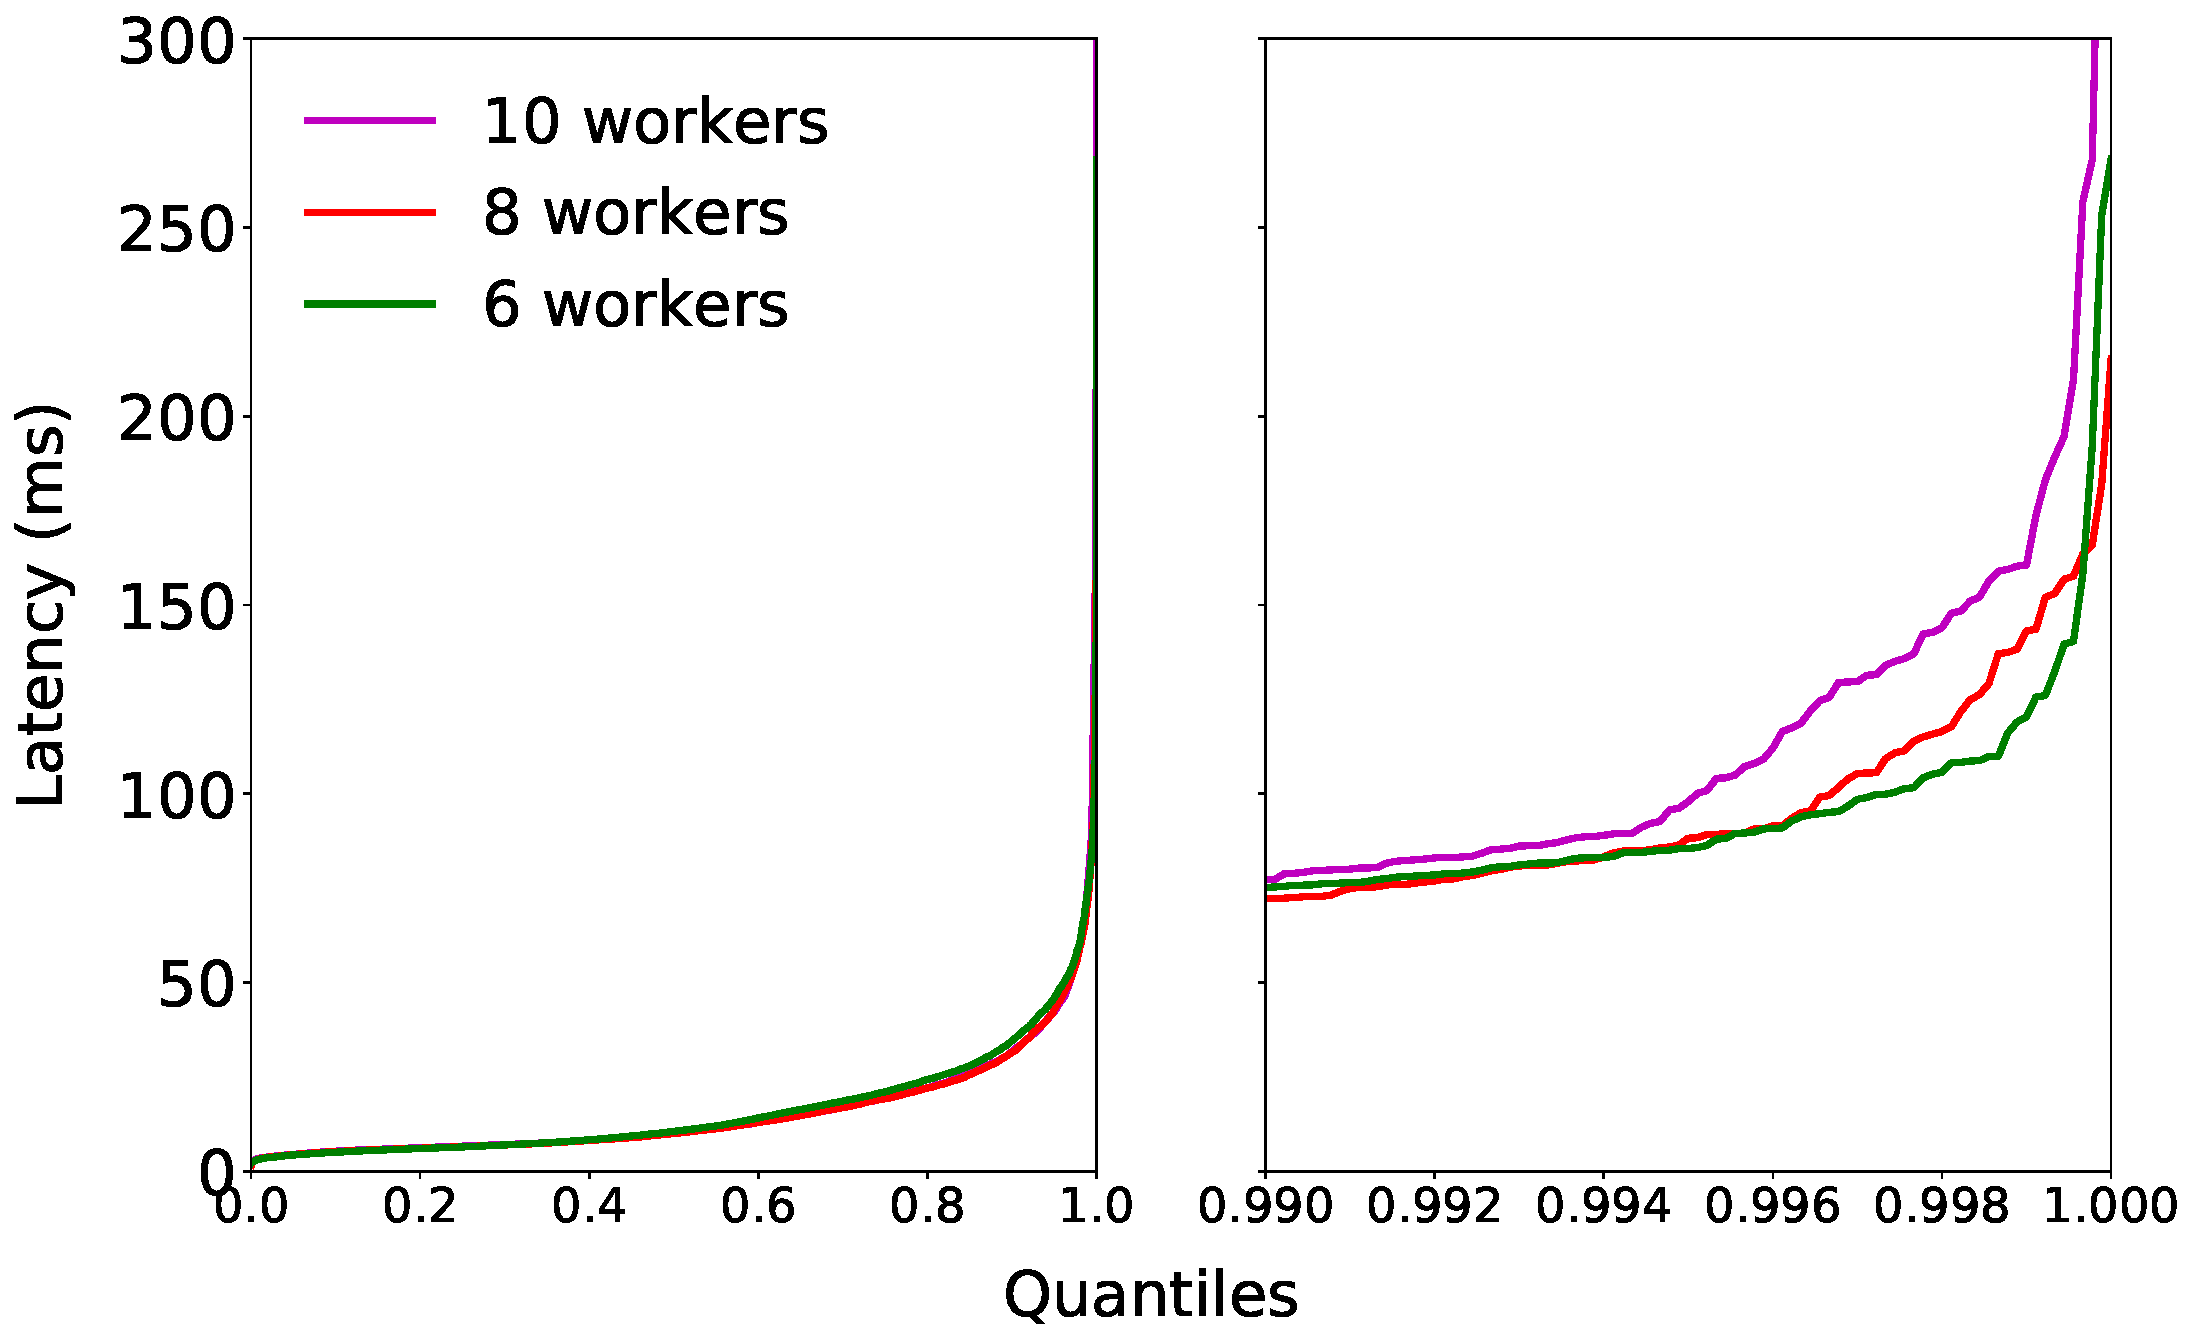
\includegraphics[width=\linewidth]{pics/fs-index-quantiles}
    \captionof{figure}{FlameStream latency distribution (left),  high quantiles (right)}
    \label{fs-scalability}
  \end{minipage}%
  \hspace{\fill}
  \begin{minipage}[b]{.40\textwidth}
    \centering
    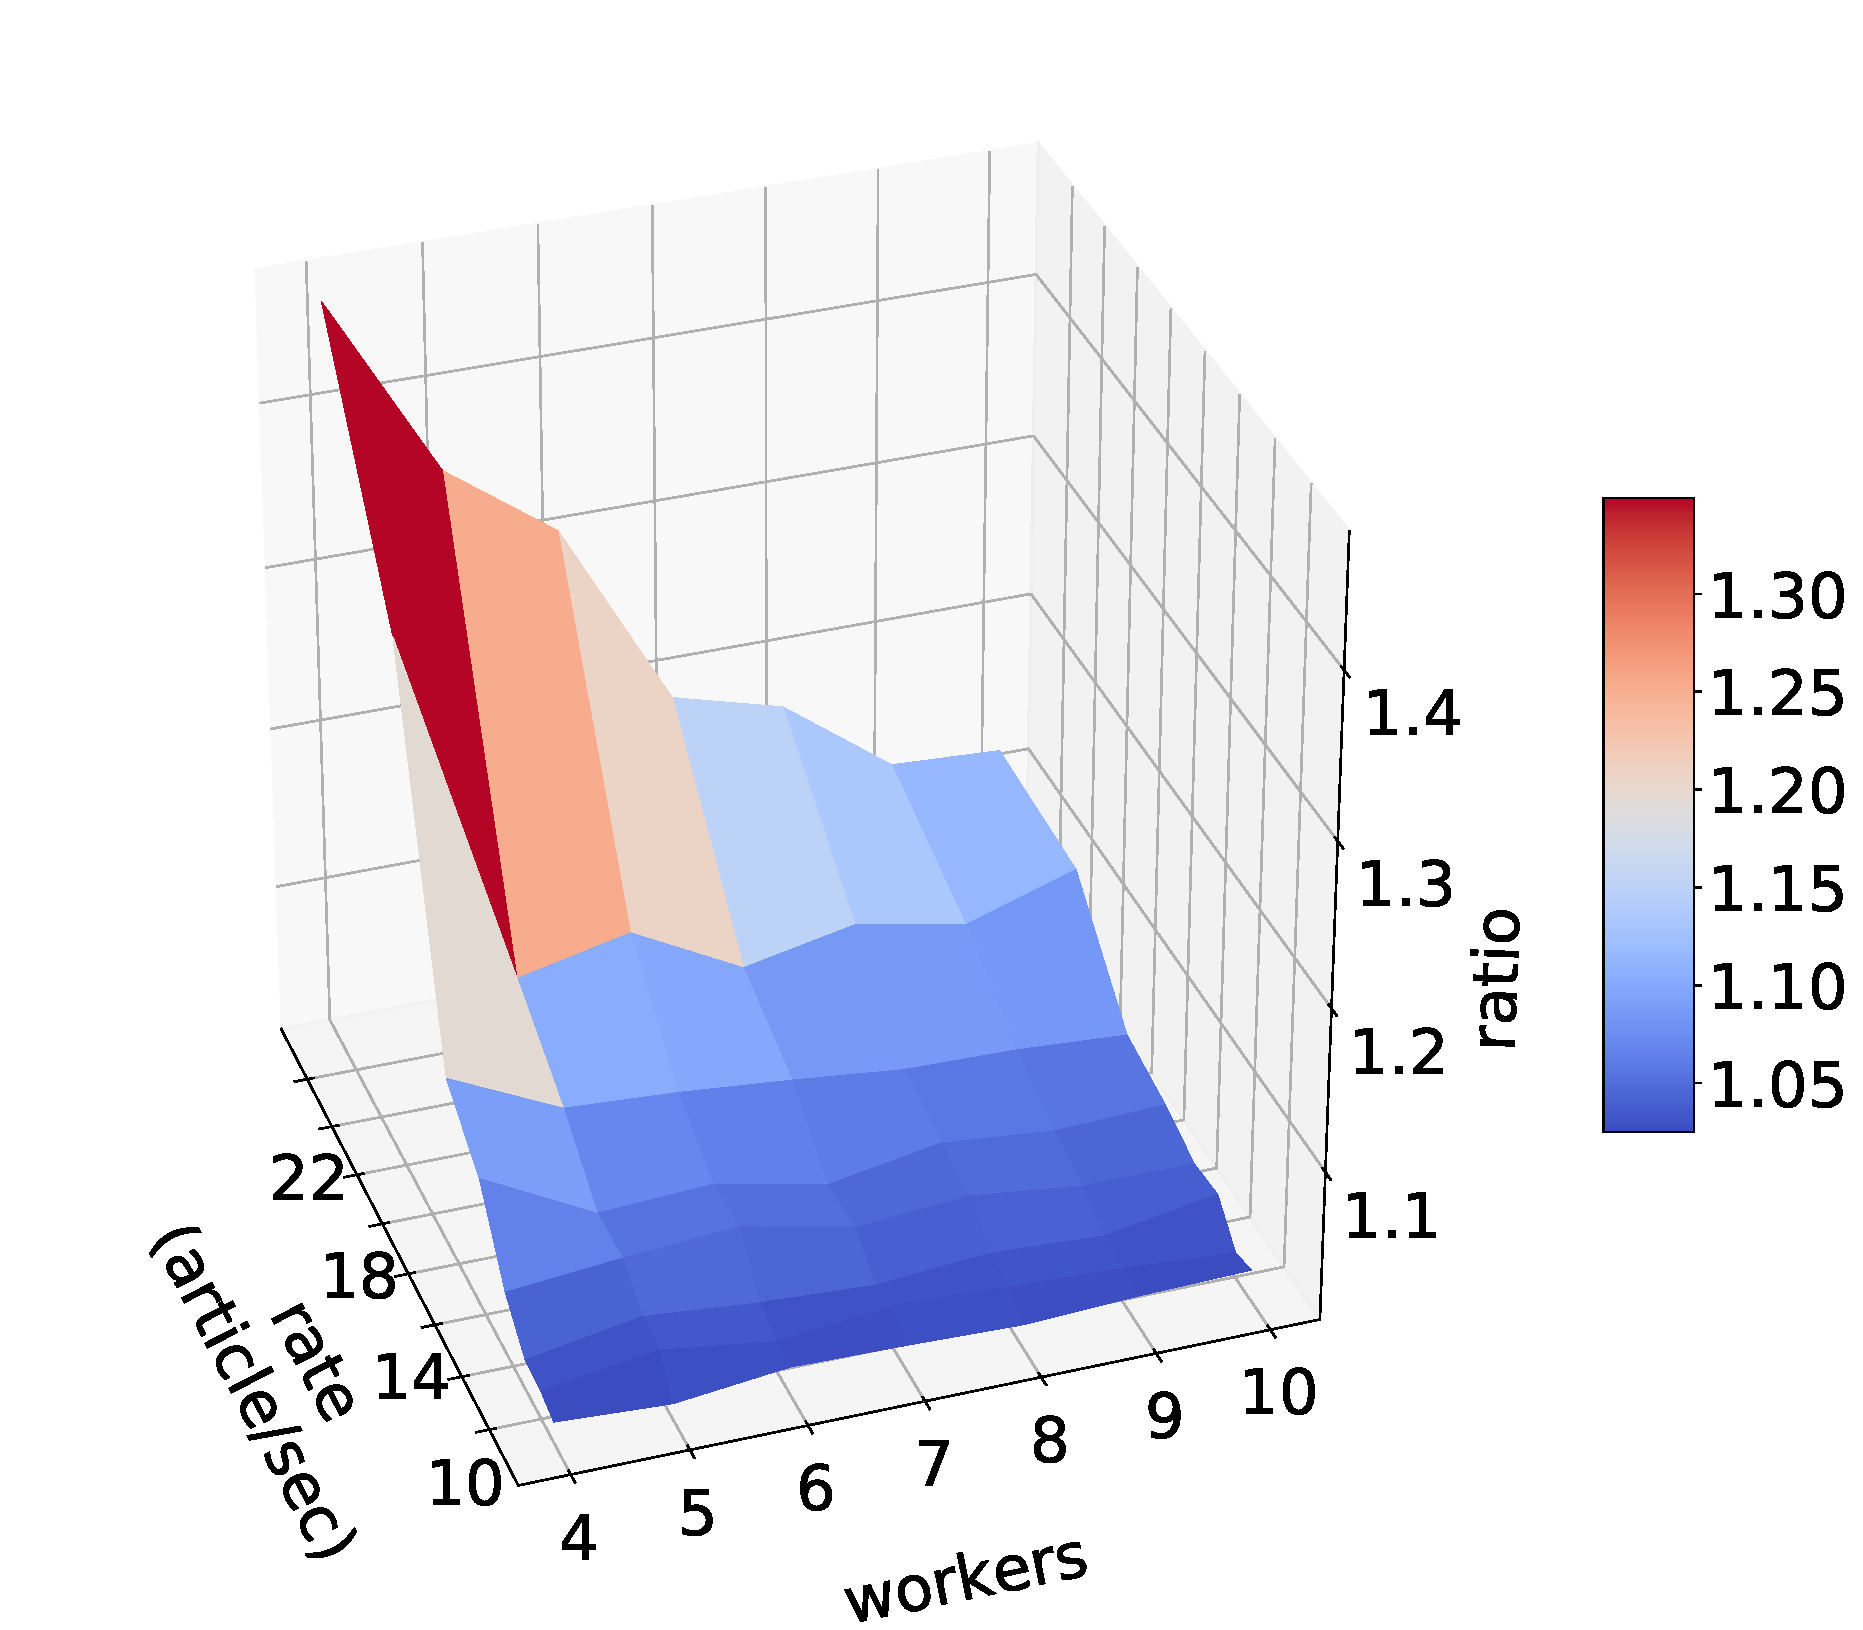
\includegraphics[width=\linewidth]{pics/overhead}
    \captionof{figure}{The relation between the number of workers, the average input rate, and the repair ratio}
    \label{overhead}
  \end{minipage}%
\end{minipage}

\begin{minipage}{\linewidth}
  \centering
  \includegraphics[width=\linewidth]{pics/comparison}
  \captionof{figure}{The comparison in latencies between FlameStream and Flink for different consistency semantics within 10 nodes and 50 documents per second input rate}
\end{minipage}

\end{multicols*}
\end{document}
